\documentclass[a4paper,12pt]{article}
\usepackage{amsmath,amssymb,amsfonts,amsthm}
\usepackage{tikz}
\usepackage [utf8x] {inputenc}
\usepackage [T2A] {fontenc} 
\usepackage[russian]{babel}
\usepackage{cmap} 
\usepackage{ gensymb }
% Так ссылки в PDF будут активны
\usepackage[unicode]{hyperref}
\usepackage{ textcomp }
\usepackage{indentfirst}
\usepackage[version=3]{mhchem}

% вы сможете вставлять картинки командой \includegraphics[width=0.7\textwidth]{ИМЯ ФАЙЛА}
% получается подключать, как минимум, файлы .pdf, .jpg, .png.
\usepackage{graphicx}
% Если вы хотите явно указать поля:
\usepackage[margin=1in]{geometry}
% Или если вы хотите задать поля менее явно (чем больше DIV, тем больше места под текст):
% \usepackage[DIV=10]{typearea}

\usepackage{fancyhdr}

\newcommand{\bbR}{\mathbb R}%теперь вместо длинной команды \mathbb R (множество вещественных чисел) можно писать короткую запись \bbR. Вместо \bbR вы можете вписать любую строчку букв, которая начинается с '\'.
\newcommand{\eps}{\varepsilon}
\newcommand{\bbN}{\mathbb N}
\newcommand{\dif}{\mathrm{d}}

\newtheorem{Def}{Определение}


\pagestyle{fancy}
\makeatletter % сделать "@" "буквой", а не "спецсимволом" - можно использовать "служебные" команды, содержащие @ в названии
\fancyhead[L]{\footnotesize Оптика}%Это будет написано вверху страницы слева
\fancyhead[R]{\footnotesize ФМХФ МФТИ}
\fancyfoot[L]{\footnotesize \@author}%имя автора будет написано внизу страницы слева
\fancyfoot[R]{\thepage}%номер страницы —- внизу справа
\fancyfoot[C]{}%по центру внизу страницы пусто

\renewcommand{\maketitle}{%
	\noindent{\bfseries\scshape\large\@title\ \mdseries\upshape}\par
	\noindent {\large\itshape\@author}
	\vskip 2ex}
\makeatother
\def\dd#1#2{\frac{\partial#1}{\partial#2}}


\title{4.2.3 \\ Интерферометр Майкельсона}
\author{Егор Берсенев} 
\date{16 февраля 2017 г.}

\begin{document}

	\maketitle
	
	\section{Цель работы} 
	Изучение двухлучевой интерференции, определение длины волны, проверка эффекта Доплера.
	
	\section{Оборудование} 
	Интерферометр Майкельсона с подвижным зеркалом, лазер ЛГН-203, фотоумножитель ФЭУ-68 с блоком питания, частотомер ЧЗ-54, линзы.
	
	\section{Теоретическое введение}
	
	\subsection{Интерференция волн двух точечных источников света}
	
	$S_1$ $(0, 0, z_1)$, $S_2$ $(0, 0, z_2)$ - изображения источника $S$, $(x, y, 0)$ - координаты точки экрана. Разность хода лучей от источников $S_1$ и $S_2$:
	
	\begin{equation}\label{eq:delta}
	\delta = \sqrt{z_1^2 + x^2 + y^2} - \sqrt{z_2^2 + x^2 + y^2}
	\end{equation}
	
	При заданной величине $\delta$ это уравнение определяет координаты $x, y$ семейства точек, обладающих одной и той же разностью хода. Наибольшая разность  хода достигается в центре интерференционной картины, в точке $O$: \[ \delta_0 = z_1 - z_2 = 2(BC - BD)\]
	В нашей установке $\delta_0 = 8 cm$. Для длины волны излучения лазера $\lambda = 0.6328 \text{ мкм}$, разности хода соответствует порядок интерференции 
	
	\begin{equation}\label{eq:order}
	m_0 = \frac{\delta_0}{\lambda} \approx 1.2\cdot10^5
	\end{equation}
	
	\begin{figure}[h!]\label{fig:inter}
		\begin{center}
			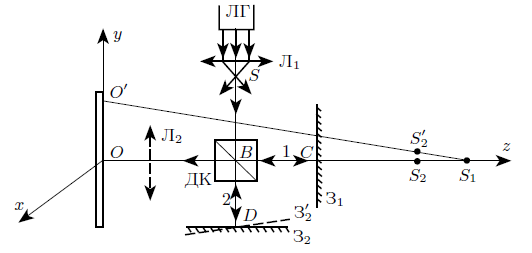
\includegraphics[width = \linewidth]{inter}
			\caption{Схема интерферометра}
		\end{center}
	\end{figure}
	
	Вблизи центра экрана выражение \eqref{eq:delta} преобразуется в:
	
	\begin{equation}\label{eq:delta_center}
	\delta \approx z_1\left(1+\frac{x^2+y^2}{2z_1^2}\right) - z_2\left(1+\frac{x^2+y^2}{2z_2^2}\right) = \delta_0 - \frac{\delta_0}{2z_1z_2}(x^2+y^2)
	\end{equation}
	
	Величина $n = (\delta - \delta_0)/\lambda$ соответствует номеру интерференционного кольца, отсчитанного от центра картины. Из \eqref{eq:order} и \eqref{eq:delta_center} следует:
	
	\begin{equation}\label{eq:rn}
	n = \frac{\delta_0}{2r_1r_2}\frac{r_n^2}{\lambda} \text{ или } r_n \approx \sqrt{\frac{2nz_1z_2}{m_0}} 
	\end{equation}
	
	При $n \gg 1$ разность $r_{n+1} - r_n$ можно заменить на $\frac{dr_n}{dn}dn$. У соседних полос $dn = 1$. Тогда расстояние между полосами:
	
	\begin{equation}\label{eq:Delta}
	\Delta = \frac{dr_n}{dn} = \sqrt{\frac{z_1z_2}{2nm_0}}
	\end{equation}
	
	При повороте зеркала $\text{З}_2$ изображение $S_2$ переходит в $S_2^{'}$ с координатами $(0, y_2, z_2)$, центр интерференционной картины переходит в точку $O^{'}$. Координата $y^{'}$ точки $O^{'}$ равна \[y^{'} = y_2\frac{z_1}{\delta_0}\].
	Для небольших углов поворота интерференционные полосы вблизи центра экрана можно приближенно считать кольцами. Номер интерференционного кольца $n_1$ можно определить, приравнивая радиус этого кольца $r_n$ смещению центра интерференционной картины $y^{'}$. Из \eqref{eq:order} и \eqref{eq:Delta}:
	
	\begin{equation}
	\begin{aligned}
	&y^{'2} = \frac{2nz_1z_2}{m_0} \text{ , } n=\frac{\delta_0y^{'2}}{2z_1z_2}\\
	&\Delta = \frac{z_1z_2\lambda}{\delta_0y^{'}} = \lambda\frac{z_2}{y_2} = \frac{\lambda}{\tan\varphi} \approx \frac{\lambda}{\varphi}
	\end{aligned}
	\end{equation}
	
	При смещении зеркала $\text{З}_1$ на расстояние $\lambda/2$ интерференционная картина восстанавливается. При смещении зеркала $\text{З}_1$ на расстояние $L$ в центре картины возникнет или исчезнет
	
	\begin{equation}\label{eq:N}
	N = 2\frac{L}{\lambda}
	\end{equation}
	
	Если при равномерном движении зеркала за время $T$ зарегистрировано возникновение или исчезновение $N$ колец, то скорость перемещения зеркала равна
	
	\begin{equation}\label{eq:speed}
	\upsilon = \frac{\lambda}{2}\frac{N}{T}
	\end{equation}  
	
	\subsection{Эффект Доплера}
	
	В системе движущегося со скоростью $\upsilon$ навстречу экрану зеркала $\text{З}_1$ частота излучения источника $\omega_1$ отличается от исходной $\omega_0$: \[ \omega_1 = \omega_0\sqrt{\frac{c+\upsilon}{c-\upsilon}} \]. Частота отраженного сигнала $\omega_2$ в ЛСО отличается от частоты $\omega_1$:
	
	\begin{equation}\label{eq:freq}
	\omega_2 = \omega_1\sqrt{\frac{c+\upsilon}{c-\upsilon}} = \omega_0\frac{c+\upsilon}{c-\upsilon}
	\end{equation}
	
	В центре экрана колебания с частотами $\omega_0$ и $\omega_2$ складываются. Суммарное колебание имеет вид: \[ E = E_0(\cos\omega_0t + \cos\omega_2t) = \left(2E_0\cos\frac{\omega_2-\omega_0}{2}t\right)\cos\frac{\omega_2+\omega_0}t{2} \]. Следовательно, регистрируемая интенсивность колебаний меняется во времени как \[ \cos^2\frac{\omega_2-\omega_0}{2}t = \frac{1+\cos(\omega_2 - \omega_0)t}{2} \], т.е. с круговой частотой
	
	\begin{equation}\label{eq:Delta_omega}
	\Delta \omega = \omega_2 - \omega_0 = \frac{2\upsilon}{c-\upsilon}\omega_0
	\end{equation}
	
	Число $N$ периодов колебаний интенсивности,  измеренное за время $T$, равно
	
	\begin{equation}\label{eq:N_rel}
	N = \frac{(\omega_2 - \omega_0)T}{2\pi} = 2\frac{\upsilon T}{\lambda}\frac{1}{1 - \frac{\upsilon}{c}} \approx \frac{2\upsilon T}{\lambda}
	\end{equation}  
	
	\section{Экспериментальная установка}
	
	\begin{figure}[h!]\label{fig:scheme}
		\begin{center}
			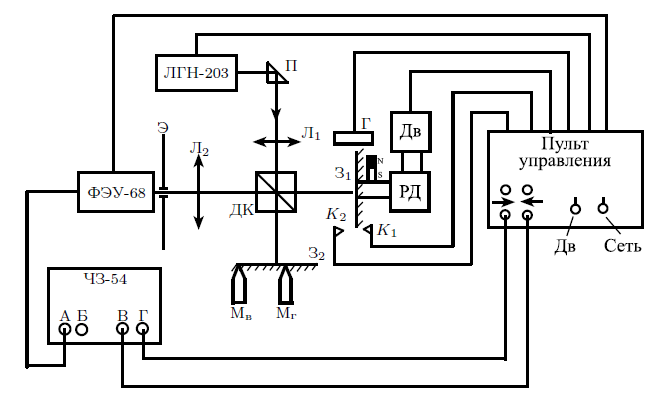
\includegraphics[width = \linewidth]{scheme}
			\caption{Схема интерферометра}
		\end{center}
	\end{figure}
	
	В нашей установке $l = 32 mm$
	
	\begin{table}[h!]\label{tab:speed}
		\centering
		\caption{Скорости движения $\text{З}_1$}
		\begin{tabular}{|c|c|c|c|c|c|}
			\hline
			№ & $t_1 \text{, ms}$ & $t_2 \text{, ms}$ & $t_3 \text{, ms}$ & $ \bar{t}  \text{, ms}$ & $\upsilon = l/\bar{t} \text{, } 10^{-3}\frac{mm}{s}$ \\ \hline
			1 & 87890 & 88160 & 88301 & $88117 \pm 121$ & $363\pm1$ \\ \hline
			2 & 39635 & 39232 & 39150 & $39339 \pm 150$ & $813\pm3$ \\ \hline
		\end{tabular}
	\end{table}
	
	\section{Эксперимент}
	
	
	\begin{table}[h!]\label{tab:frequency}
		\begin{minipage}[]{0.54\textwidth}
			\centering
			\caption{$\upsilon = \upsilon_1$}
			\resizebox{\textwidth}{!}{%
				\begin{tabular}[b]{|c|c|c|c|c|c|}
					\hline
					\multicolumn{6}{|c|}{$N/T, \text{ kHz}$} \\ \hline
					\multicolumn{3}{|c|}{от экрана} & \multicolumn{3}{c|}{к экрану} \\ \hline
					1.112 & 1.149 & 1.151 & 1.158 & 1.186 & 1.137 \\ \hline
					1.28 & 1.139 & 1.159 & 1.164 & 1.16 & 1.16 \\ \hline
					1.138 & 1.126 & 1.131 & 1.163 & 1.153 & 1159 \\ \hline
					1.124 & 1.145 & 1.157 & 1.161 & 1.165 & 1.156 \\ \hline
					1.131 & 1.129 & 1.111 & 1.171 & 1.173 & 1.172 \\ \hline
					1.135 & 1.131 & 1.129 & 1.159 & 1.157 & 1.182 \\ \hline
					1.155 & 1.156 & 1.137 & 1.183 & 1.163 & 1.171 \\ \hline
					1.145 & 1.149 & 1.119 & 1.187 & 1.154 & 1.15 \\ \hline
					1.139 & 1.122 & 1.141 & 1.176 & 1.159 & 1.164 \\ \hline
					1.162 & 1.151 & 1.122 & 1.168 & 1.175 & 1.15 \\ \hline
					1.13 & 1.124 &  & 1.174 & 1.17 & 1.186 \\ \hline
					1.143 & 1.141 &  & 1.168 & 1.165 & 1.159 \\ \hline
					1.149 & 1.158 &  & 1.167 & 1.164 & 1.12 \\ \hline
					1.124 & 1.136 &  & 1.173 & 1.178 & 1.155 \\ \hline
					1.132 & 1.137 &  & 1.158 & 1.149 & 1.163 \\ \hline
					1.165 & 1.138 &  & 1.142 & 1.145 & 1.125 \\ \hline
					1.121 & 1.118 &  & 1.159 & 1.139 & 1.144 \\ \hline
					1.135 & 1.118 &  & 1.162 & 1.172 &  \\ \hline
				\end{tabular}%
			}
		\end{minipage}
		\hfill
		\begin{minipage}{0.4\textwidth}
			\centering
			\caption{$\upsilon = \upsilon_2$}
			\resizebox{\textwidth}{!}{%
				\begin{tabular}{|c|c|c|c|}
					\hline
					\multicolumn{4}{|c|}{$N/T, \text{ kHz}$} \\ \hline
					\multicolumn{2}{|c|}{от экрана} & \multicolumn{2}{c|}{к экрану} \\ \hline
					2.633 & 2.608 & 2.518 & 2.533 \\ \hline
					2.599 & 2.568 & 2.522 & 2.566 \\ \hline
					2.584 & 2.601 & 2.579 & 2.582 \\ \hline
					2.605 & 2.572 & 2.603 & 2.625 \\ \hline
					2.571 & 2.563 & 2.623 & 2.644 \\ \hline
					2.539 & 2.539 & 2.663 & 2.63 \\ \hline
					2.555 & 2.549 & 2.62 & 2.628 \\ \hline
					2.566 & 2.523 & 2.632 & 2.631 \\ \hline
					2.636 & 2.69 & 2.478 & 2.509 \\ \hline
					2.619 & 2.657 & 2.579 & 2.558 \\ \hline
					2.609 & 2.636 & 2.592 & 2.576 \\ \hline
					2.615 & 2.63 & 2.628 & 2.495 \\ \hline
					2.581 & 2.608 & 2.669 & 2.67 \\ \hline
					2.563 & 2.577 & 2.657 & 2.66 \\ \hline
					2.537 & 2.608 & 2.643 & 2.68 \\ \hline
					2.557 & 2.595 & 2.64 & 2.679 \\ \hline
				\end{tabular}%
			}
		\end{minipage}
	\end{table}		
	
	Для малых скоростей $\upsilon$ формула \eqref{eq:N_rel} справедлива и в случае отдаляющегося от экрана зеркала $\text{З}_1$. Найдем средние значения частот колебания интенсивности интерференционной картины и оценим погрешности.
	
	\begin{table}[h!]\label{tab:freq}
		\centering
		\caption{Средние частоты}
		\begin{tabular}{|c|c|c|}
			\hline
			\multicolumn{3}{|c|}{$\langle N/T \rangle \text{ ,kHz}$} \\ \hline
			$\upsilon$ & от экрана & к экрану \\ \hline
			$\upsilon_1$ & $1.137\pm0.002$ & $1.162\pm0.002$ \\ \hline
			$\upsilon_2$ & $2.590\pm0.001$ & $2.603\pm0.01$ \\ \hline
		\end{tabular}
	\end{table}
	
	Построим графики зависимости доплеровской частоты от скорости передвижения зеркала. Из графиков находим
	
	$$
	\lambda_{from} = 0.6349 \pm 0.0051 \, \text{nm} $$$$
	\lambda_{to} = 0.6250 \pm 0.0002 \, \text{nm}
	$$
	
	\begin{figure}[h!]\label{fig:lambda}
		\begin{center}
			\begin{minipage}{0.49\textwidth}
				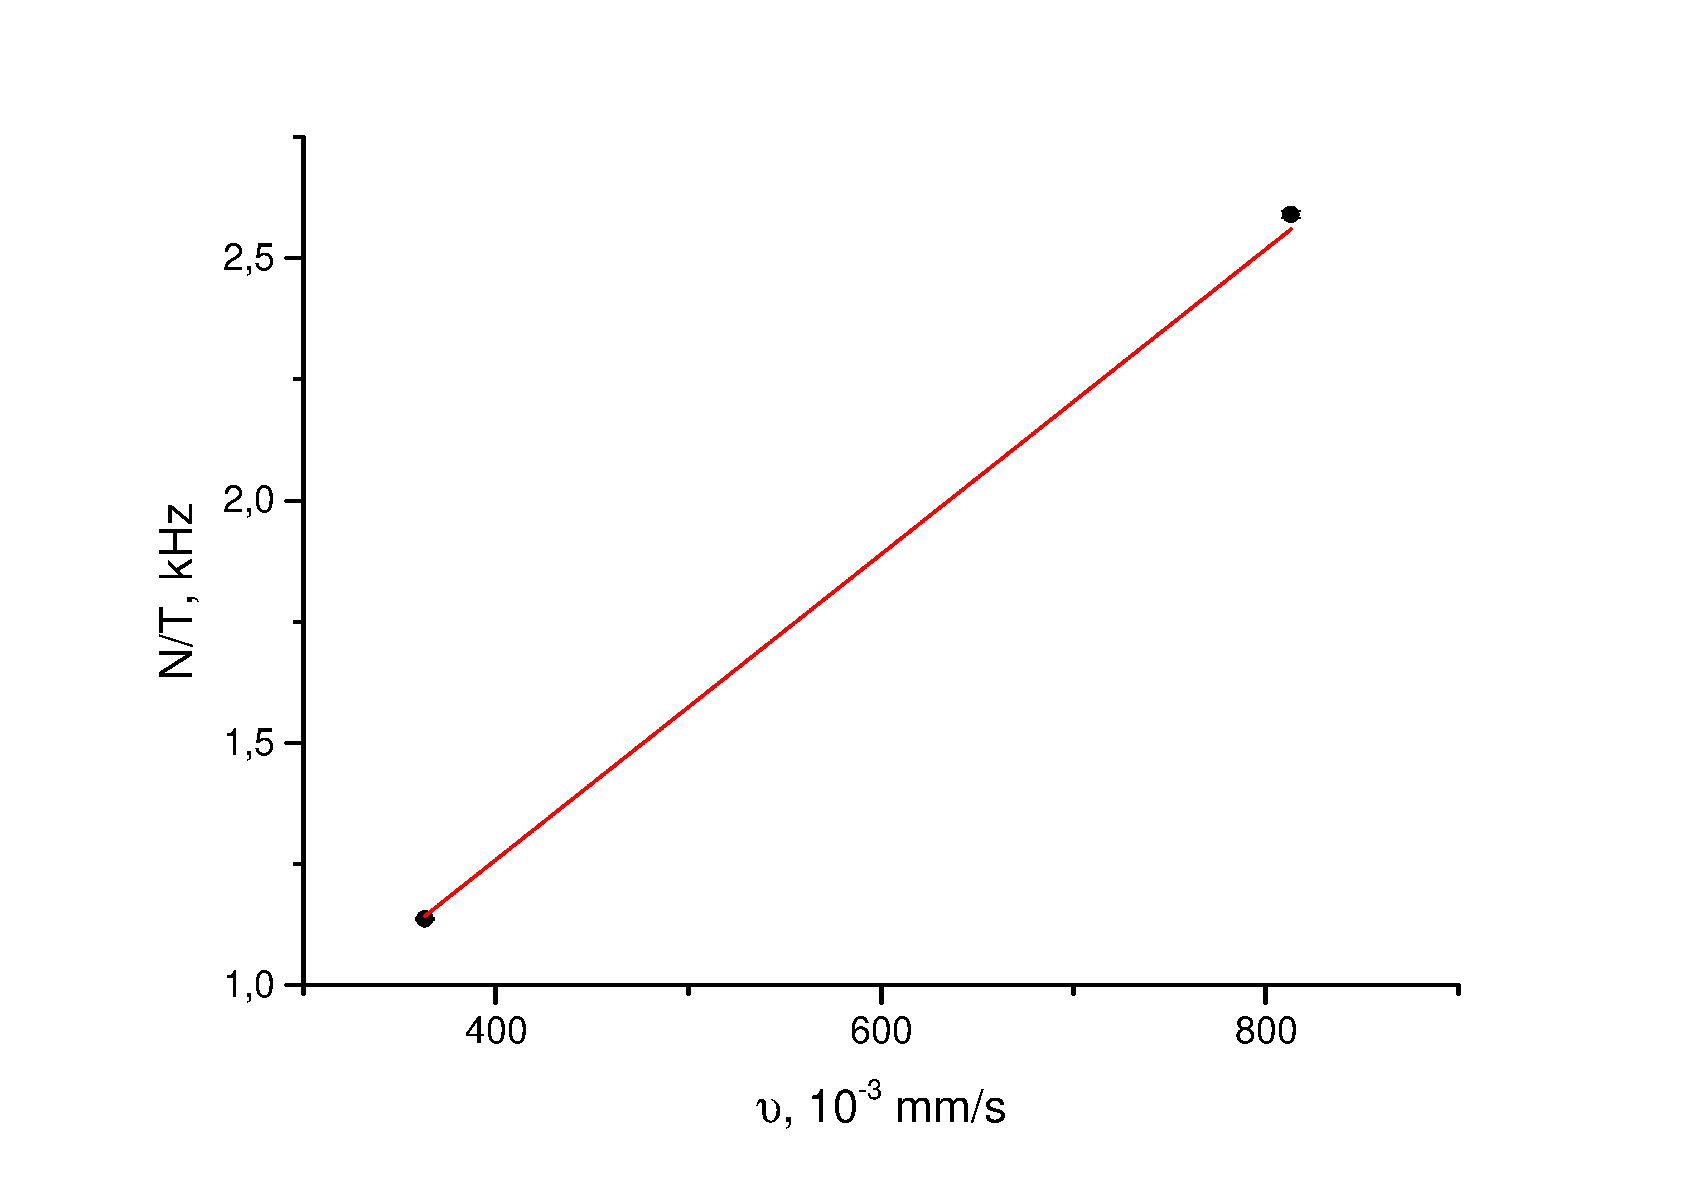
\includegraphics[width=\textwidth]{fs}
				\caption{от экрана}
			\end{minipage}
			\hfill
			\begin{minipage}{0.49\textwidth}
				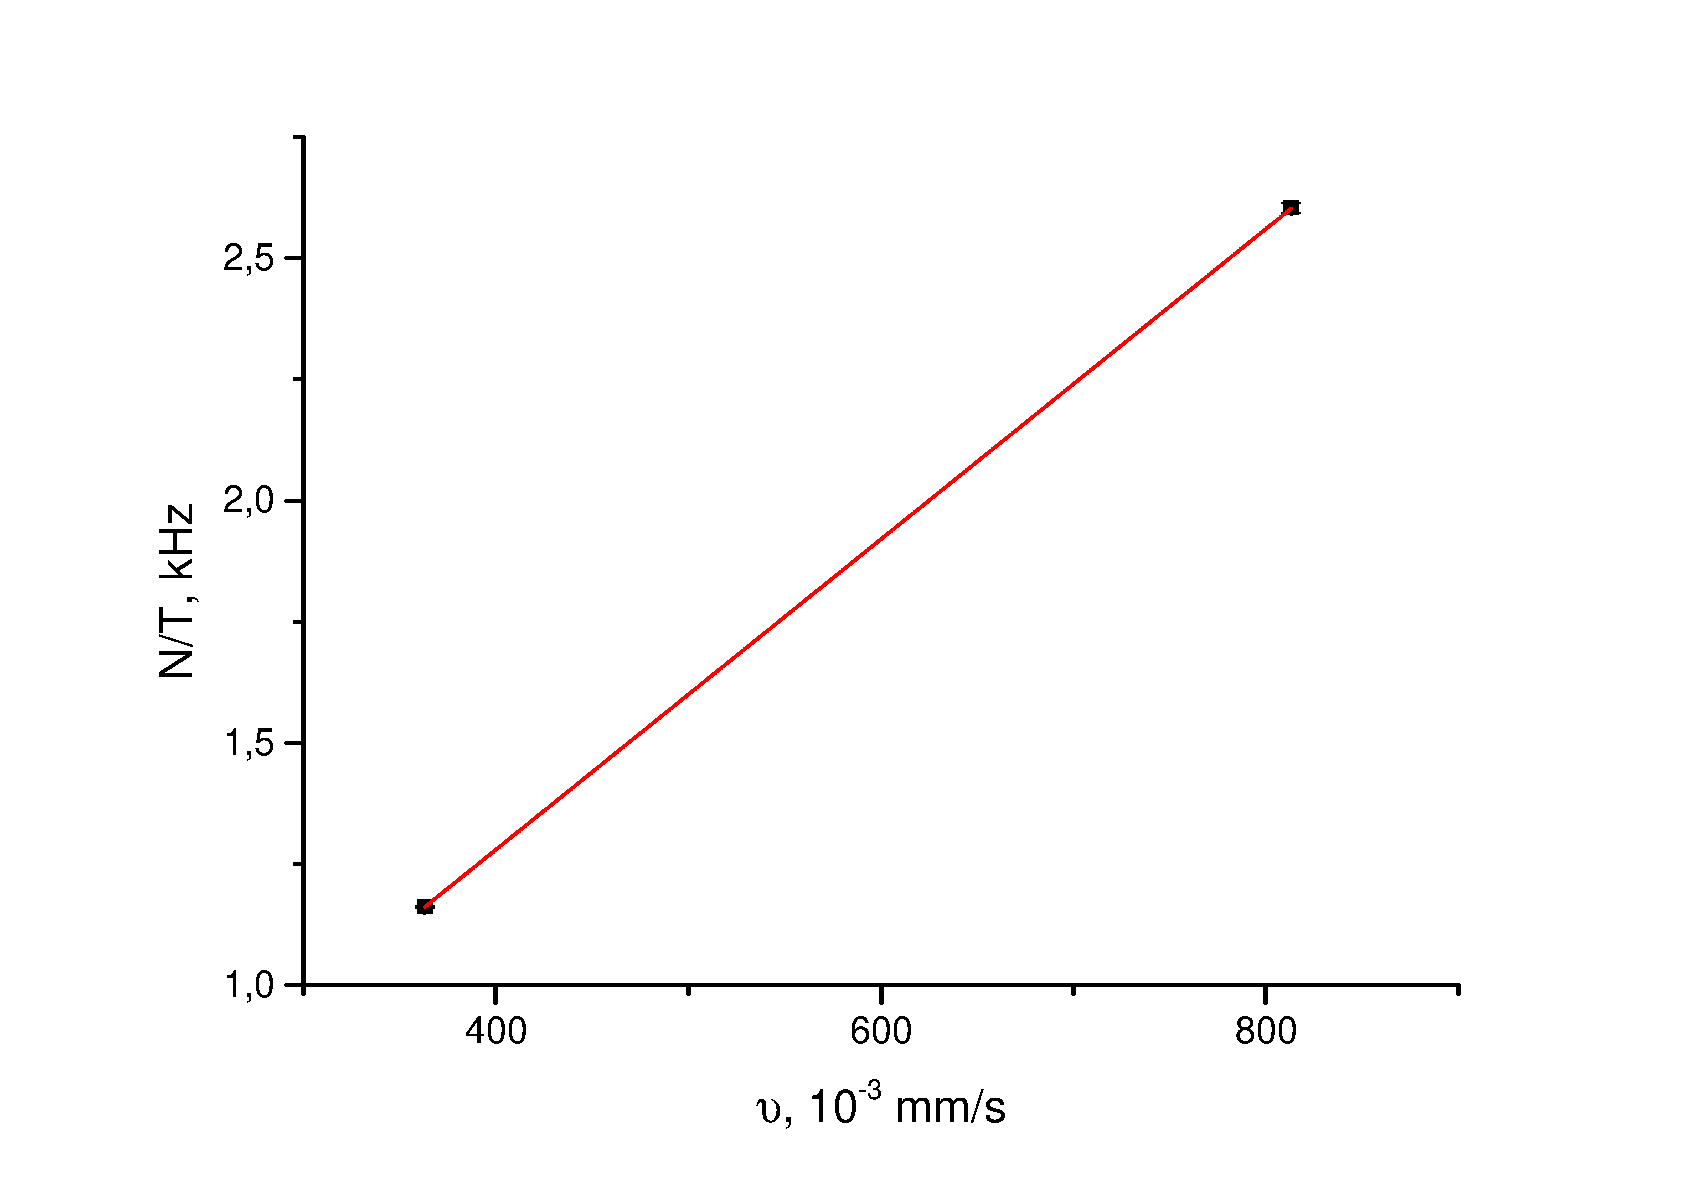
\includegraphics[width=\textwidth]{ts}
				\caption{к экрану}
			\end{minipage}
		\end{center}
	\end{figure}
	
	Полученные значения совпадают с фактической длиной волны лазера в нашей установке. Значит, формула \eqref{eq:N_rel} справедлива.
	
	\begin{figure}[h!]\label{fig:picture}
		\begin{center}
			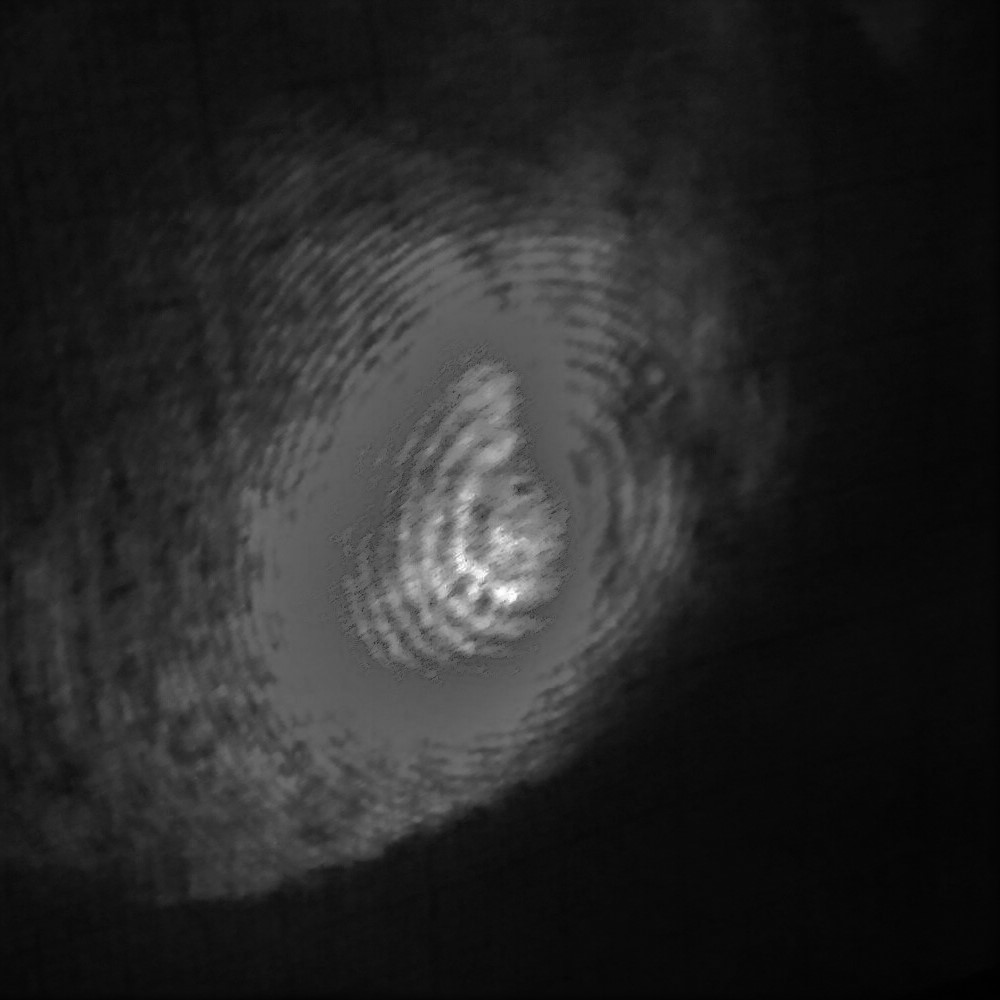
\includegraphics[width = 0.3\linewidth]{picture}
			\caption{Интерференционная картина}
		\end{center}
	\end{figure}
	
	\section{Вывод}
	
	В проделанной работе была получена интерференционная картина двухлучевой интерференции. Также была экспериментально определена длина волны источника и проверен эффект Доплера.
\end{document}


